\documentclass[a4paper,12pt]{extarticle}

\usepackage[T2A]{fontenc}
\usepackage[utf8]{inputenc}
\usepackage[english,russian]{babel}
\usepackage{geometry}
\usepackage{setspace}
\usepackage{indentfirst}
\usepackage{titlesec}
\usepackage{graphicx}
\usepackage{amsmath,amssymb}
\usepackage{booktabs,array}
\usepackage{caption}
\usepackage{placeins}
\usepackage[nottoc]{tocbibind}
\usepackage[hidelinks]{hyperref}

\geometry{a4paper,left=30mm,top=30mm,bottom=30mm,right=30mm}
\onehalfspacing
\graphicspath{{img/}{figures/}}
\hypersetup{
    pdftitle={Параллельное решение задачи Дирихле для уравнения Пуассона},
    pdfauthor={Аристархов Данила Дмитриевич}
}
\addto\captionsrussian{\renewcommand{\refname}{Литература}}
\captionsetup{font=small}
\setlength{\emergencystretch}{2em}
\widowpenalty=10000
\clubpenalty=10000
\renewcommand{\arraystretch}{1.15}

\begin{document}

\begin{titlepage}
    \centering
    
\includegraphics[width=10.5cm]{msu_logo.pdf}

    \large
    Московский государственный университет имени М.В. Ломоносова\\
    Факультет вычислительной математики и кибернетики\\
    Кафедра математических методов прогнозирования

    \vspace{1.0in}
    Аристархов Данила Дмитриевич\\
    Группа 617

    \vspace{0.35in}
    {\bfseries
    Параллельное решение задачи Дирихле\\
    для уравнения Пуассона\par}

    \vspace{0.35in}
    ОТЧЁТ ПО ЗАДАНИЮ №\,1\\
    Вариант 3

    \vspace{0.25in}
    Курс <<Суперкомпьютерное моделирование\\
    и технологии>>

    \vfill
    {\bfseries Москва, 2026}
\end{titlepage}

\setcounter{page}{2}
\tableofcontents
\newpage

\section{Введение}

В работе рассматривается численное решение задачи Дирихле для уравнения Пуассона в трапеции. Для этого используются метод фиктивных областей, пятиточечная разностная схема и метод сопряжённых градиентов с диагональным предобусловливателем.

Были разработаны последовательная программа и реализации OpenMP, MPI и MPI+OpenMP. Их корректность и скорость были проверены на IBM Polus при различных размерах сетки и числе процессов и потоков.

\section{Постановка задачи}

Согласно варианту 3 задания~\cite{task}, областью $D$ является трапеция с вершинами $(0,0)$, $(3,0)$, $(2,3)$ и $(0,3)$. Тогда
\[
    D=\left\{(x,y)\colon 0<y<3,\quad 0<x<3-\frac{y}{3}\right\}.
\]
Требуется найти функцию $u(x,y)$, удовлетворяющую уравнению
\begin{equation}
    -\Delta u=1,\qquad (x,y)\in D,
    \label{eq:poisson}
\end{equation}
и граничному условию
\begin{equation}
    u(x,y)=\sin(x+y),\qquad (x,y)\in\partial D.
    \label{eq:boundary}
\end{equation}
Для построения равномерной сетки выберем прямоугольник $\Pi=(-1,4)\times(-1,4)$, содержащий замыкание $D$. Исходная и расчётная области представлены на рис.~\ref{fig:geometry}.

\begin{figure}[!htbp]
    \centering
    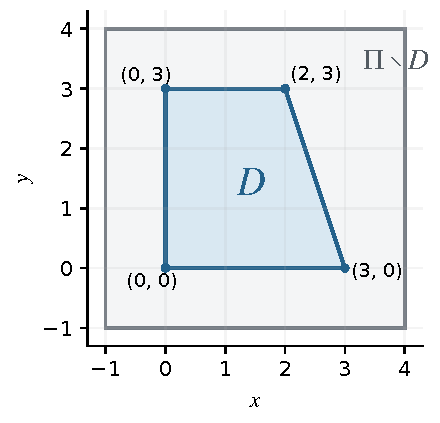
\includegraphics[width=0.40\textwidth]{geometry.pdf}
    \caption{Трапеция $D$ и прямоугольник $\Pi$}
    \label{fig:geometry}
\end{figure}
\FloatBarrier

\section{Численный метод}

\subsection{Метод фиктивных областей}

Продолжим граничную функцию на весь прямоугольник: $g(x,y)=\sin(x+y)$. Вместо задачи~\eqref{eq:poisson}--\eqref{eq:boundary} будем решать задачу
\begin{equation}
    -\Delta v+Q(x,y)\bigl(v-g(x,y)\bigr)=F(x,y),
    \qquad v|_{\partial\Pi}=g,
    \label{eq:fictitious}
\end{equation}
где
\[
    Q(x,y)=
    \begin{cases}
        0, & (x,y)\in D,\\
        \varepsilon^{-2}, & (x,y)\in\Pi\setminus D,
    \end{cases}
    \qquad
    F(x,y)=
    \begin{cases}
        1, & (x,y)\in D,\\
        0, & (x,y)\in\Pi\setminus D.
    \end{cases}
\]

Внутри трапеции уравнение~\eqref{eq:fictitious} совпадает с исходным. В фиктивной области слагаемое $Q(v-g)$ ограничивает отклонение $v$ от $g$. При уменьшении $\varepsilon$ это позволяет приближённо выполнить условие Дирихле на границе трапеции. Таким образом, задачу в области со скошенной стороной можно решать на прямоугольной сетке.

Коэффициент $Q$ имеет разрыв на $\partial D$, однако он входит в уравнение как множитель и не дифференцируется. Для заданного $\varepsilon>0$ он ограничен и неотрицателен, поэтому разрыв не нарушает положительную определённость оператора. В соответствии с заданием используется $\varepsilon=h^2$, где $h$ --- наибольший шаг сетки.

\subsection{Разностная схема}

Разобьём стороны прямоугольника на $M$ и $N$ интервалов. Узлы сетки и её шаги определяются следующим образом:
\[
    h_x=\frac{5}{M},\qquad h_y=\frac{5}{N},\qquad
    x_i=-1+ih_x,\qquad y_j=-1+jh_y.
\]
Здесь $i=0,\ldots,M$, $j=0,\ldots,N$. Далее обозначение сетки $M\times N$ соответствует числу интервалов по каждой координате. Общее число узлов равно $(M+1)(N+1)$, а число внутренних узлов --- $(M-1)(N-1)$.

Для каждого внутреннего узла рассмотрим прямоугольную ячейку $\Pi_{ij}$ с центром в $(x_i,y_j)$ и сторонами $h_x$, $h_y$. Коэффициенты разностной схемы определим как средние по этой ячейке:
\[
    Q_{ij}=\frac{1}{h_xh_y}\iint_{\Pi_{ij}}Q(x,y)\,dx\,dy,
    \qquad
    F_{ij}=\frac{1}{h_xh_y}\iint_{\Pi_{ij}}F(x,y)\,dx\,dy.
\]
Пусть $S_{ij}$ --- площадь пересечения $\Pi_{ij}$ с трапецией. Тогда, обозначив долю ячейки внутри области через $\theta_{ij}$, получаем
\begin{equation}
    \theta_{ij}=\frac{S_{ij}}{h_xh_y},\qquad
    F_{ij}=\theta_{ij},\qquad
    Q_{ij}=\frac{1-\theta_{ij}}{\varepsilon^2}.
    \label{eq:coefficients}
\end{equation}

На каждом уровне $y$ правая граница трапеции равна $3-y/3$, поэтому ширина пересечения с ячейкой является кусочно-линейной функцией. Площадь $S_{ij}$ вычисляется интегрированием этой ширины: интервал разбивается в точках смены формулы, а на каждом участке применяется формула трапеций. Для данной области такой способ даёт точную площадь с учётом ошибок округления.

Заменяя вторые производные центральными разностями, получаем
\begin{equation}
\begin{split}
    -\frac{w_{i-1,j}-2w_{ij}+w_{i+1,j}}{h_x^2}
    -\frac{w_{i,j-1}-2w_{ij}+w_{i,j+1}}{h_y^2}
    +Q_{ij}w_{ij}\\
    =F_{ij}+Q_{ij}g(x_i,y_j).
\end{split}
    \label{eq:scheme}
\end{equation}
На внешней границе прямоугольника значения $w_{ij}$ известны. Перенесём их в правую часть и оставим неизвестными только значения во внутренних узлах. В результате получим СЛАУ $Aw=B$ с диагональными элементами
\[
    d_{ij}=\frac{2}{h_x^2}+\frac{2}{h_y^2}+Q_{ij}.
\]
Коэффициенты при соседях по $x$ и $y$ равны соответственно $-h_x^{-2}$ и $-h_y^{-2}$. Например, при $i=1$ в правую часть добавляется $g(-1,y_j)/h_x^2$.

Матрица $A$ симметрична и положительно определена. Поэтому для решения системы можно использовать метод сопряжённых градиентов. Саму матрицу целиком хранить не требуется: её действие на вектор вычисляется по пятиточечному шаблону.

\subsection{Метод сопряжённых градиентов}

Введём скалярное произведение и норму сеточных функций:
\[
    (a,b)_h=h_xh_y\sum_{i=1}^{M-1}\sum_{j=1}^{N-1}a_{ij}b_{ij},
    \qquad
    \|a\|_h=\sqrt{(a,a)_h}.
\]
В качестве предобусловливателя выберем $K=\operatorname{diag}(A)$. Тогда вычисление $K^{-1}r$ сводится к делению каждого элемента невязки на соответствующий диагональный коэффициент.

Начальное приближение задаётся нулевым. Начальные невязка и направление поиска имеют вид
\[
    w^0=0,\qquad r^0=B,\qquad z^0=K^{-1}r^0,\qquad p^0=z^0.
\]
На очередной итерации сначала вычисляются
\[
    \rho_k=(r^k,z^k)_h,\qquad
    \alpha_k=\frac{\rho_k}{(p^k,Ap^k)_h}.
\]
После этого обновляются решение и невязка:
\[
    w^{k+1}=w^k+\alpha_kp^k,\qquad
    r^{k+1}=r^k-\alpha_kAp^k.
\]
Новое направление определяется формулами
\begin{align*}
    z^{k+1}&=K^{-1}r^{k+1},\qquad
    \beta_k=\frac{(r^{k+1},z^{k+1})_h}{\rho_k},\\
    p^{k+1}&=z^{k+1}+\beta_kp^k.
\end{align*}

В качестве условия остановки используется
\begin{equation}
    \|w^{k+1}-w^k\|_h<\delta,\qquad \delta=10^{-8}.
    \label{eq:stop}
\end{equation}
Также процесс заканчивается при нулевой невязке. Число итераций ограничено числом неизвестных.

Для контроля сходимости на каждом шаге вычисляется функционал
\[
    J(w)=\frac12(Aw,w)_h-(B,w)_h=-\frac12(B+r,w)_h.
\]
Если его значение увеличивается сверх допуска на ошибки округления, восстанавливается предыдущее приближение, заново вычисляется невязка и выполняется перезапуск метода. Для уменьшения ошибок суммирования в скалярных произведениях используется алгоритм Кэхэна. В проведённых расчётах перезапуски не потребовались.

\section{Параллельная реализация}

Во всех версиях программы используются одна разностная схема и один итерационный метод. Основные операции на каждой итерации --- применение оператора $A$, обновление векторов и вычисление скалярных произведений. Именно эти операции были распараллелены.

\subsection{OpenMP}

В OpenMP-версии данные находятся в общей памяти. Между потоками распределяются циклы по узлам сетки при вычислении коэффициентов и применении оператора, а также циклы обновления векторов. Для распределения итераций используется \texttt{schedule(static)}, поскольку объём работы в каждом узле примерно одинаков.

При вычислении скалярного произведения каждый поток сначала находит локальную сумму с компенсацией ошибок округления. Затем частичные суммы объединяются с помощью редукции OpenMP. Итерации самого метода сопряжённых градиентов не распараллеливаются, т.к. очередное приближение зависит от предыдущего.

\subsection{MPI}

Для MPI-версии прямоугольная сетка разбивается на $p_x\times p_y$ блоков, где $p_xp_y=P$, а $P$ --- число процессов. Число узлов по каждой координате в разных блоках отличается не более чем на единицу. Разбиение выбирается так, чтобы отношение количества узлов по двум координатам в каждом домене принадлежало отрезку $[1/2,2]$. Например, для сетки $800\times1200$ и 32 процессов используется решётка $4\times8$.

Каждый процесс хранит значения в своём блоке и дополнительный слой соседних узлов. Перед применением оператора $A$ выполняется обмен крайними строками и столбцами с соседними процессами. Для этого используется \texttt{MPI\_Sendrecv}; столбцы передаются с помощью типа, созданного через \texttt{MPI\_Type\_vector}.

Скалярное произведение сначала вычисляется на локальном блоке, после чего частичные суммы объединяются через \texttt{MPI\_Allreduce}. Полное решение собирается только после завершения итераций для записи в файл. На границах между блоками используются значения соседнего процесса, а условия Дирихле задаются только на внешней границе прямоугольника.

\subsection{MPI+OpenMP}

В гибридной версии сохраняется то же разбиение между MPI-процессами. Внутри каждого блока локальные циклы распределяются между OpenMP-потоками. Таким образом, MPI отвечает за обмен данными между блоками, а OpenMP --- за вычисления внутри блока.

Вызовы MPI выполняются основным потоком вне параллельных областей. Для этого при инициализации запрашивается уровень \texttt{MPI\_THREAD\_FUNNELED}. Число потоков $T$ задаётся отдельно для каждого процесса; после запуска проверяется, что оно одинаково на всех процессах и совпадает с требуемым.

\section{Эксперименты}

\subsection{Условия проведения экспериментов}

Расчёты были выполнены на IBM Polus. Узел этой системы содержит два процессора IBM POWER8 по 10 физических ядер. Каждое ядро поддерживает до восьми аппаратных потоков~\cite{polus}.

Программы написаны на C++11 и собраны компилятором GCC~4.8.5 с оптимизацией \texttt{-O2}. Для OpenMP использовался флаг \texttt{-fopenmp}, для MPI --- библиотека SpectrumMPI. Запуск выполнялся через очередь \texttt{normal} планировщика LSF.

Последовательной программе выделялось одно ядро. Для OpenMP выделялось 16 физических ядер одного узла, поэтому при 32 потоках использовался SMT. Для MPI выделялось до 32 процессов, не более 16 на узел. В гибридной версии использовалось до четырёх процессов по восемь ядер, не более двух процессов на узел~\cite{polus_omp,polus_hybrid}.

Время измерялось вокруг вызова решателя. Оно включает инициализацию его рабочих векторов, итерации и итоговый пересчёт невязки. Подготовка сетки, запуск процессов и запись решения в это время не входят. В MPI-версиях за время решения принимался максимум по всем процессам.

Ускорение рассчитывалось относительно последовательной программы на той же сетке:
\begin{equation}
    S=\frac{t_{\mathrm{seq}}}{t_{\mathrm{par}}}.
    \label{eq:speedup}
\end{equation}
Для каждой конфигурации в итоговых таблицах использован один замер. Гибридные результаты получены из повторной серии, в которой на всех процессах было проверено заданное число потоков.

\subsection{Проверка корректности}

Сначала были выполнены последовательные расчёты на сетках $20\times20$, $40\times40$ и $80\times80$. Для сравнения времени параллельных программ также были проведены последовательные расчёты на сетках из приложения к заданию. Их результаты представлены в табл.~\ref{tab:seq}. Относительная невязка вычислялась после завершения итераций как $\|B-Aw\|_h/\|B\|_h$.

\begin{table}[htbp]
    \centering
    \begin{singlespace}
    \small
    \begin{tabular}{rrrr}
        \toprule
        Сетка & Итерации & Время, с & Относительная невязка\\
        \midrule
        $20\times20$ & 39 & $0{,}000512$ & $3{,}68\cdot10^{-10}$\\
        $40\times40$ & 77 & $0{,}004171$ & $1{,}02\cdot10^{-10}$\\
        $80\times80$ & 151 & $0{,}033462$ & $1{,}83\cdot10^{-11}$\\
        $400\times600$ & 892 & $19{,}018$ & $5{,}10\cdot10^{-13}$\\
        $800\times1200$ & 1736 & $149{,}500$ & $1{,}20\cdot10^{-13}$\\
        \bottomrule
    \end{tabular}
    \end{singlespace}
    \caption{Результаты последовательной программы}
    \label{tab:seq}
\end{table}

Для проверки параллельных реализаций были проведены расчёты на сетке $80\times80$. В табл.~\ref{tab:check} приведено максимальное отклонение от последовательного решения в узлах сетки. Во всех конфигурациях потребовалась 151 итерация; расхождение не превысило $2{,}00\cdot10^{-15}$.

\begin{table}[htbp]
    \centering
    \begin{singlespace}
    \small
    \begin{tabular}{lrrrr}
        \toprule
        Реализация & $P$ & $T$ & Время, с & $\max |w-w_{\mathrm{seq}}|$\\
        \midrule
        OpenMP & 1 & 1 & $0{,}036651$ & $0$\\
        OpenMP & 1 & 4 & $0{,}015255$ & $1{,}44\cdot10^{-15}$\\
        OpenMP & 1 & 16 & $0{,}025387$ & $2{,}00\cdot10^{-15}$\\
        MPI & 1 & 1 & $0{,}018643$ & $0$\\
        MPI & 2 & 1 & $0{,}010612$ & $1{,}55\cdot10^{-15}$\\
        MPI & 4 & 1 & $0{,}006490$ & $1{,}44\cdot10^{-15}$\\
        MPI+OpenMP & 1 & 4 & $0{,}009551$ & $1{,}44\cdot10^{-15}$\\
        MPI+OpenMP & 2 & 4 & $0{,}009342$ & $1{,}44\cdot10^{-15}$\\
        \bottomrule
    \end{tabular}
    \end{singlespace}
    \caption{Сравнение реализаций на сетке $80\times80$}
    \label{tab:check}
\end{table}

На больших сетках максимальное расхождение OpenMP- и MPI-решений с последовательным составило $2{,}58\cdot10^{-14}$. В итоговой гибридной серии число итераций совпало с последовательной программой, а относительная невязка не превысила $5{,}11\cdot10^{-13}$ на сетке $400\times600$ и $1{,}21\cdot10^{-13}$ на сетке $800\times1200$.

Также сравнивались решения на сгущающихся сетках. Максимальная разность в общих узлах внутри $\overline D$ составила $0{,}075148$ при переходе от $20\times20$ к $40\times40$ и $0{,}030068$ при переходе от $40\times40$ к $80\times80$. Для сеток $400\times600$ и $800\times1200$ эта разность равна $0{,}007113$. Различия уменьшаются при сгущении, однако они характеризуют разность сеточных приближений, а не ошибку относительно точного решения.

На рис.~\ref{fig:solution} представлено решение на наибольшей сетке $800\times1200$. Значения в фиктивной области не показаны.

\begin{figure}[htbp]
    \centering
    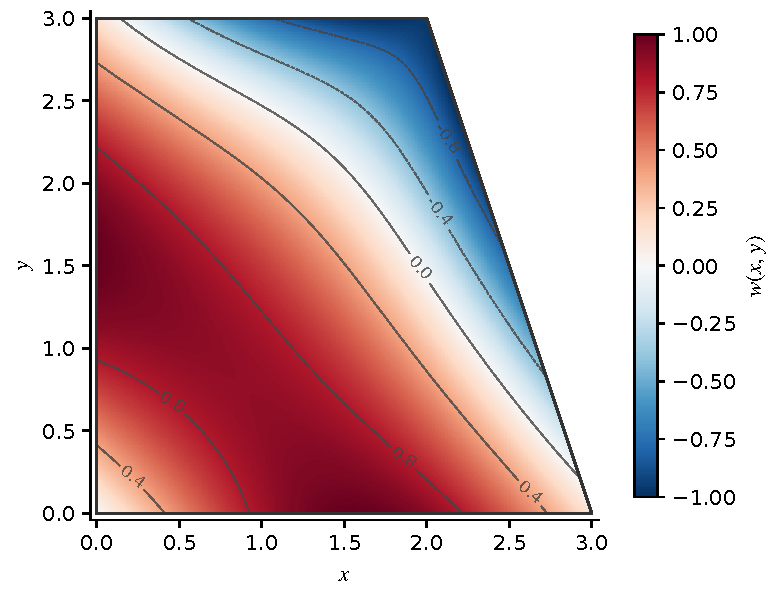
\includegraphics[width=0.80\textwidth]{solution.pdf}
    \caption{Приближённое решение на сетке $800\times1200$}
    \label{fig:solution}
\end{figure}

\FloatBarrier

\clearpage
\subsection{OpenMP}

Результаты OpenMP-программы приведены в табл.~\ref{tab:omp}, зависимость ускорения от числа потоков --- на рис.~\ref{fig:omp}. Увеличение числа потоков уменьшает время решения на обеих сетках. При этом число итераций не меняется, т.е. ускорение связано с параллельным выполнением операций одной итерации.

\begin{table}[htbp]
    \centering
    \begin{singlespace}
    \small
    \begin{tabular}{rrrrr}
        \toprule
        Потоки & Сетка & Итерации & Время, с & Ускорение\\
        \midrule
        2 & $400\times600$ & 892 & $8{,}161$ & $2{,}330$\\
        4 & $400\times600$ & 892 & $4{,}103$ & $4{,}635$\\
        8 & $400\times600$ & 892 & $2{,}133$ & $8{,}917$\\
        16 & $400\times600$ & 892 & $1{,}150$ & $16{,}544$\\
        \midrule
        4 & $800\times1200$ & 1736 & $31{,}990$ & $4{,}673$\\
        8 & $800\times1200$ & 1736 & $16{,}123$ & $9{,}273$\\
        16 & $800\times1200$ & 1736 & $8{,}199$ & $18{,}235$\\
        32 & $800\times1200$ & 1736 & $5{,}201$ & $28{,}742$\\
        \bottomrule
    \end{tabular}
    \end{singlespace}
    \caption{Результаты OpenMP-программы}
    \label{tab:omp}
\end{table}

\begin{figure}[htbp]
    \centering
    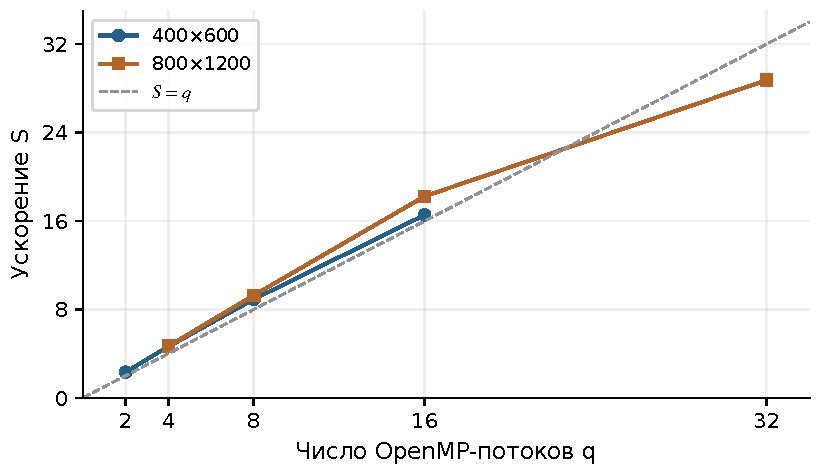
\includegraphics[width=0.90\textwidth]{speedup_omp.pdf}
    \caption{Ускорение OpenMP в зависимости от числа потоков. Пунктир: $S=q$}
    \label{fig:omp}
\end{figure}

На сетке $800\times1200$ переход от 16 к 32 потокам уменьшил время с $8{,}199$ до $5{,}201$~с. Таким образом, использование SMT дало дополнительное ускорение в $1{,}576$ раза на тех же 16 физических ядрах.
\FloatBarrier

\clearpage
\subsection{MPI}

Для MPI-программы результаты представлены в табл.~\ref{tab:mpi} и на рис.~\ref{fig:mpi}. На сетке $400\times600$ минимальное время составило $1{,}143$~с при 16 процессах. На сетке $800\times1200$ наименьшее время равно $4{,}696$~с при 32 процессах, что соответствует ускорению $31{,}836$ относительно последовательной программы.

\begin{table}[htbp]
    \centering
    \begin{singlespace}
    \small
    \begin{tabular}{rrrrr}
        \toprule
        Процессы & Сетка & Итерации & Время, с & Ускорение\\
        \midrule
        2 & $400\times600$ & 892 & $6{,}919$ & $2{,}749$\\
        4 & $400\times600$ & 892 & $4{,}500$ & $4{,}226$\\
        8 & $400\times600$ & 892 & $1{,}889$ & $10{,}069$\\
        16 & $400\times600$ & 892 & $1{,}143$ & $16{,}642$\\
        \midrule
        4 & $800\times1200$ & 1736 & $27{,}271$ & $5{,}482$\\
        8 & $800\times1200$ & 1736 & $14{,}101$ & $10{,}602$\\
        16 & $800\times1200$ & 1736 & $7{,}019$ & $21{,}299$\\
        32 & $800\times1200$ & 1736 & $4{,}696$ & $31{,}836$\\
        \bottomrule
    \end{tabular}
    \end{singlespace}
    \caption{Результаты MPI-программы}
    \label{tab:mpi}
\end{table}

\begin{figure}[htbp]
    \centering
    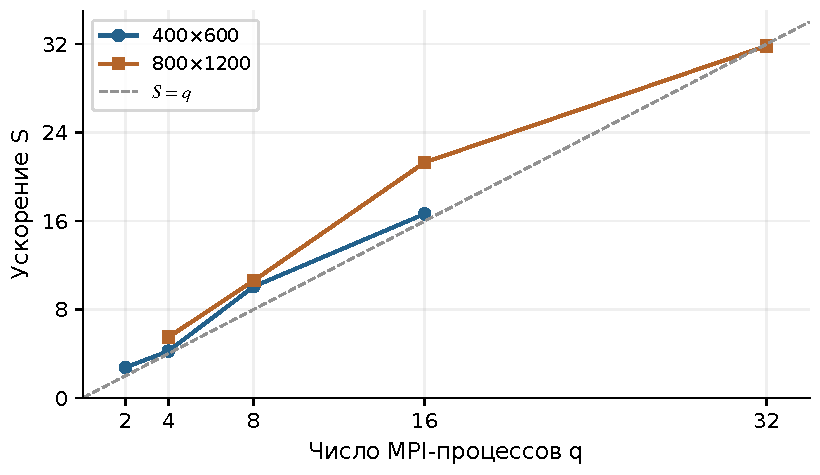
\includegraphics[width=0.90\textwidth]{speedup_mpi.pdf}
    \caption{Ускорение MPI-программы в зависимости от числа процессов}
    \label{fig:mpi}
\end{figure}

При переходе от 16 к 32 процессам на большой сетке время уменьшилось в $1{,}495$ раза. При таком разбиении локальный объём вычислений сокращается, а относительная стоимость обменов граничными значениями и глобальных редукций возрастает. Это может ограничивать дальнейшее ускорение.
\FloatBarrier

\clearpage
\subsection{MPI+OpenMP}

В гибридной версии число MPI-процессов фиксировалось: $P=2$ для сетки $400\times600$ и $P=4$ для сетки $800\times1200$. Число потоков $T$ в каждом процессе изменялось от 1 до 8. Результаты приведены в табл.~\ref{tab:hybrid} и на рис.~\ref{fig:hybrid}.

\begin{table}[htbp]
    \centering
    \begin{singlespace}
    \small
    \begin{tabular}{rrrrrr}
        \toprule
        $P$ & $T$ & Сетка & Итерации & Время, с & Ускорение\\
        \midrule
        2 & 1 & $400\times600$ & 892 & $8{,}164$ & $2{,}330$\\
        2 & 2 & $400\times600$ & 892 & $4{,}102$ & $4{,}636$\\
        2 & 4 & $400\times600$ & 892 & $2{,}090$ & $9{,}102$\\
        2 & 8 & $400\times600$ & 892 & $1{,}085$ & $17{,}524$\\
        \midrule
        4 & 1 & $800\times1200$ & 1736 & $37{,}608$ & $3{,}975$\\
        4 & 2 & $800\times1200$ & 1736 & $18{,}803$ & $7{,}951$\\
        4 & 4 & $800\times1200$ & 1736 & $9{,}566$ & $15{,}629$\\
        4 & 8 & $800\times1200$ & 1736 & $4{,}942$ & $30{,}253$\\
        \bottomrule
    \end{tabular}
    \end{singlespace}
    \caption{Результаты гибридной программы}
    \label{tab:hybrid}
\end{table}

\begin{figure}[htbp]
    \centering
    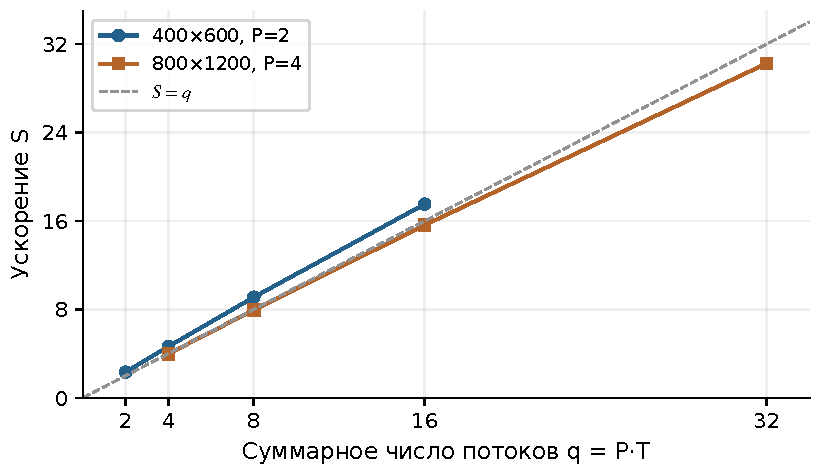
\includegraphics[width=0.90\textwidth]{speedup_hybrid.pdf}
    \caption{Ускорение MPI+OpenMP в зависимости от общего числа потоков $q=PT$}
    \label{fig:hybrid}
\end{figure}

На сетке $400\times600$ минимальное время составило $1{,}085$~с при двух процессах по восемь потоков. На сетке $800\times1200$ конфигурация из четырёх процессов по восемь потоков дала время $4{,}942$~с и ускорение $30{,}253$. Переход от четырёх к восьми потокам в каждом процессе сократил время в $1{,}936$ раза.
\FloatBarrier

\subsection{Сравнение реализаций}

При переходе от $400\times600$ к $800\times1200$ число неизвестных выросло с $239\,001$ до $958\,001$, примерно в четыре раза. Число итераций увеличилось с 892 до 1736. Поэтому рост последовательного времени в $7{,}86$ раза связан как с увеличением сетки, так и с увеличением числа итераций.

Наибольшее ускорение на сетке $800\times1200$ показала MPI-версия с 32 процессами: $31{,}836$. Гибридная версия при том же общем числе потоков дала ускорение $30{,}253$, а OpenMP --- $28{,}742$. При сравнении нужно учитывать, что OpenMP использовал 16 физических ядер с SMT, а максимальные MPI- и гибридная конфигурации использовали 32 ядра на нескольких узлах.

В отдельных конфигурациях ускорение оказалось выше числа процессов или потоков. Это может быть связано с изменением работы кэшей и памяти при разбиении данных, а также с различиями условий запуска. Поскольку для каждой конфигурации использован один замер, по полученным результатам нельзя отдельно оценить влияние этих факторов.

\section{Выводы}

В работе были реализованы последовательный и три параллельных алгоритма решения задачи Дирихле в трапеции. Для перехода к прямоугольной сетке использовался метод фиктивных областей, а полученная СЛАУ решалась методом сопряжённых градиентов с диагональным предобусловливателем.

Проверка на малой сетке показала совпадение параллельных решений с последовательным с точностью до ошибок округления. На больших сетках все реализации сошлись за одинаковое число итераций без перезапусков метода. Увеличение числа процессов и потоков позволило сократить время решения на сетке $800\times1200$ со $149{,}500$~с до $5{,}201$~с для OpenMP, $4{,}696$~с для MPI и $4{,}942$~с для MPI+OpenMP.

Наилучшее время на большой сетке было получено для MPI-версии с 32 процессами. Гибридная реализация показала близкий результат, а OpenMP позволил получить ускорение $28{,}742$ на одном узле.

\clearpage
\begin{thebibliography}{9}
    \bibitem{task}
    Мокин А.Ю. Задание по курсу <<Суперкомпьютерное моделирование и технологии>>. Сентябрь 2026.

    \bibitem{polus}
    IBM Polus. Вычислительный комплекс ВМК МГУ.
    \url{https://hpc.cs.msu.ru/polus}.

    \bibitem{polus_omp}
    Запуск OpenMP-программ на IBM Polus.
    \url{https://hpc.cs.msu.ru/node/254}.

    \bibitem{polus_hybrid}
    Запуск MPI+OpenMP-программ на IBM Polus.
    \url{https://hpc.cs.msu.ru/node/258}.
\end{thebibliography}

\end{document}
